
\chapter{无门与哥德尔}

\section{什么是禅宗?}

我不敢肯定我知道禅宗是什么。一方面,我觉得我对禅宗非常明了;但另一方面,我又觉得我永远也没法明白它。自从我大学一年级的语文老师在课堂上给我们大声朗读赵州的“无”,我就开始与禅宗式的生活观进行搏斗,也许我永远也不会停止这么做。对我来说,禅宗是智力流沙——晦涩、无意义、紊乱、无法无天。它撩人而又令人恼火。不过它也很幽默,让人耳目一新,富于吸引力。禅宗是有其特殊的意义、光芒和明晰性的。我希望在这一章里能把我的这些感受传达一些给读者。这样(虽然这似乎挺奇怪),我们就被直接引向哥德尔的理论了。

佛教禅宗的基本教条之一是:没有任何办法能刻划禅宗是什么。无论你用什么样的词语空间努力去涵盖禅宗,都不会成功,它总要再冒出去。看起来,阐释禅宗的所有努力似乎完全都是浪费时间。但禅宗信徒们并不这么看。比如说,禅宗的公案,虽然是用词语表达的,乃是禅宗探究的中心部分。公案是当作“触发器”的,它们自己并不含有足够的信息以得到顿悟,但它们可能足以解开人们心智中导致顿悟的机制。不过一般说来,禅宗的观点认为词语与真理是不相容的,或至少是词语不能捕捉到真理。

\section{无门禅师}

也许就是为了以一种极端的方式指出这一点,无门禅师在十三世纪时编辑了四十八个公案,并于每个公案后面附了评注及一首小“颂”。这部作品被称为《无门之门》,或《无门关》。有趣的是,无门与斐波那契的生活年代几乎完全相同:无门从1183年至1260年生活在中国,斐波那契于1180年到1250年生活在意大利。对于那些希望通过《无门关》而看懂或“理解”公案的人,看了《无门关》之后大概会惊诧不已:那些评注及诗句本应是澄清公案的意思的,实际上却和公案本身一样晦涩。看这个例子:\note{保罗·李普士,《禅肉,禅骨》,第110--111页。中译文出自《禅宗无门关》。}

\begin{zenkoan}
公案:
清凉大法眼,因僧斋前上参,眼以手指帘,时有二僧同去卷帘。
眼曰:“一得,一失。”
无门曰:
\begin{zenkoan}
且道:是谁得谁失?若向者里着得一只眼,便知清凉国师败阙处。然虽如此,却忌向得失里商量!
\end{zenkoan}
颂曰:
\begin{zenkoan}
卷起明明彻太空,太空犹未合吾宗。
争似从空都放下?绵绵密密不通风!
\end{zenkoan}
\end{zenkoan}
现在我们再来看一个:\note{李普士书,第119页。中译文出自《禅宗无门关》。}

\begin{zenkoan}
公案:
五祖曰:“譬如水牯牛过窗棂,头,角,四蹄都过了,因什么尾巴过不得?”
无门曰:
\begin{zenkoan}
若向者里颠倒着一只眼,下得一转语,可以上报四恩,下资三有。其或未然,更须照顾尾巴始得!
\end{zenkoan}
颂曰:
\begin{zenkoan}
过去堕坑堑,回来却被坏。
者些尾巴子,直是甚奇怪!
\end{zenkoan}
\end{zenkoan}

我想你得承认,无门并没有真的把每件事都澄清。可以说,元语言(无门用的语言)与对象语言(公案的语言)没有什么太大差别。在有些人看来,无门的那些评注纯属故意装傻,也许就是为了表明花时间谈论禅宗是毫无用处的。

\begin{figure}
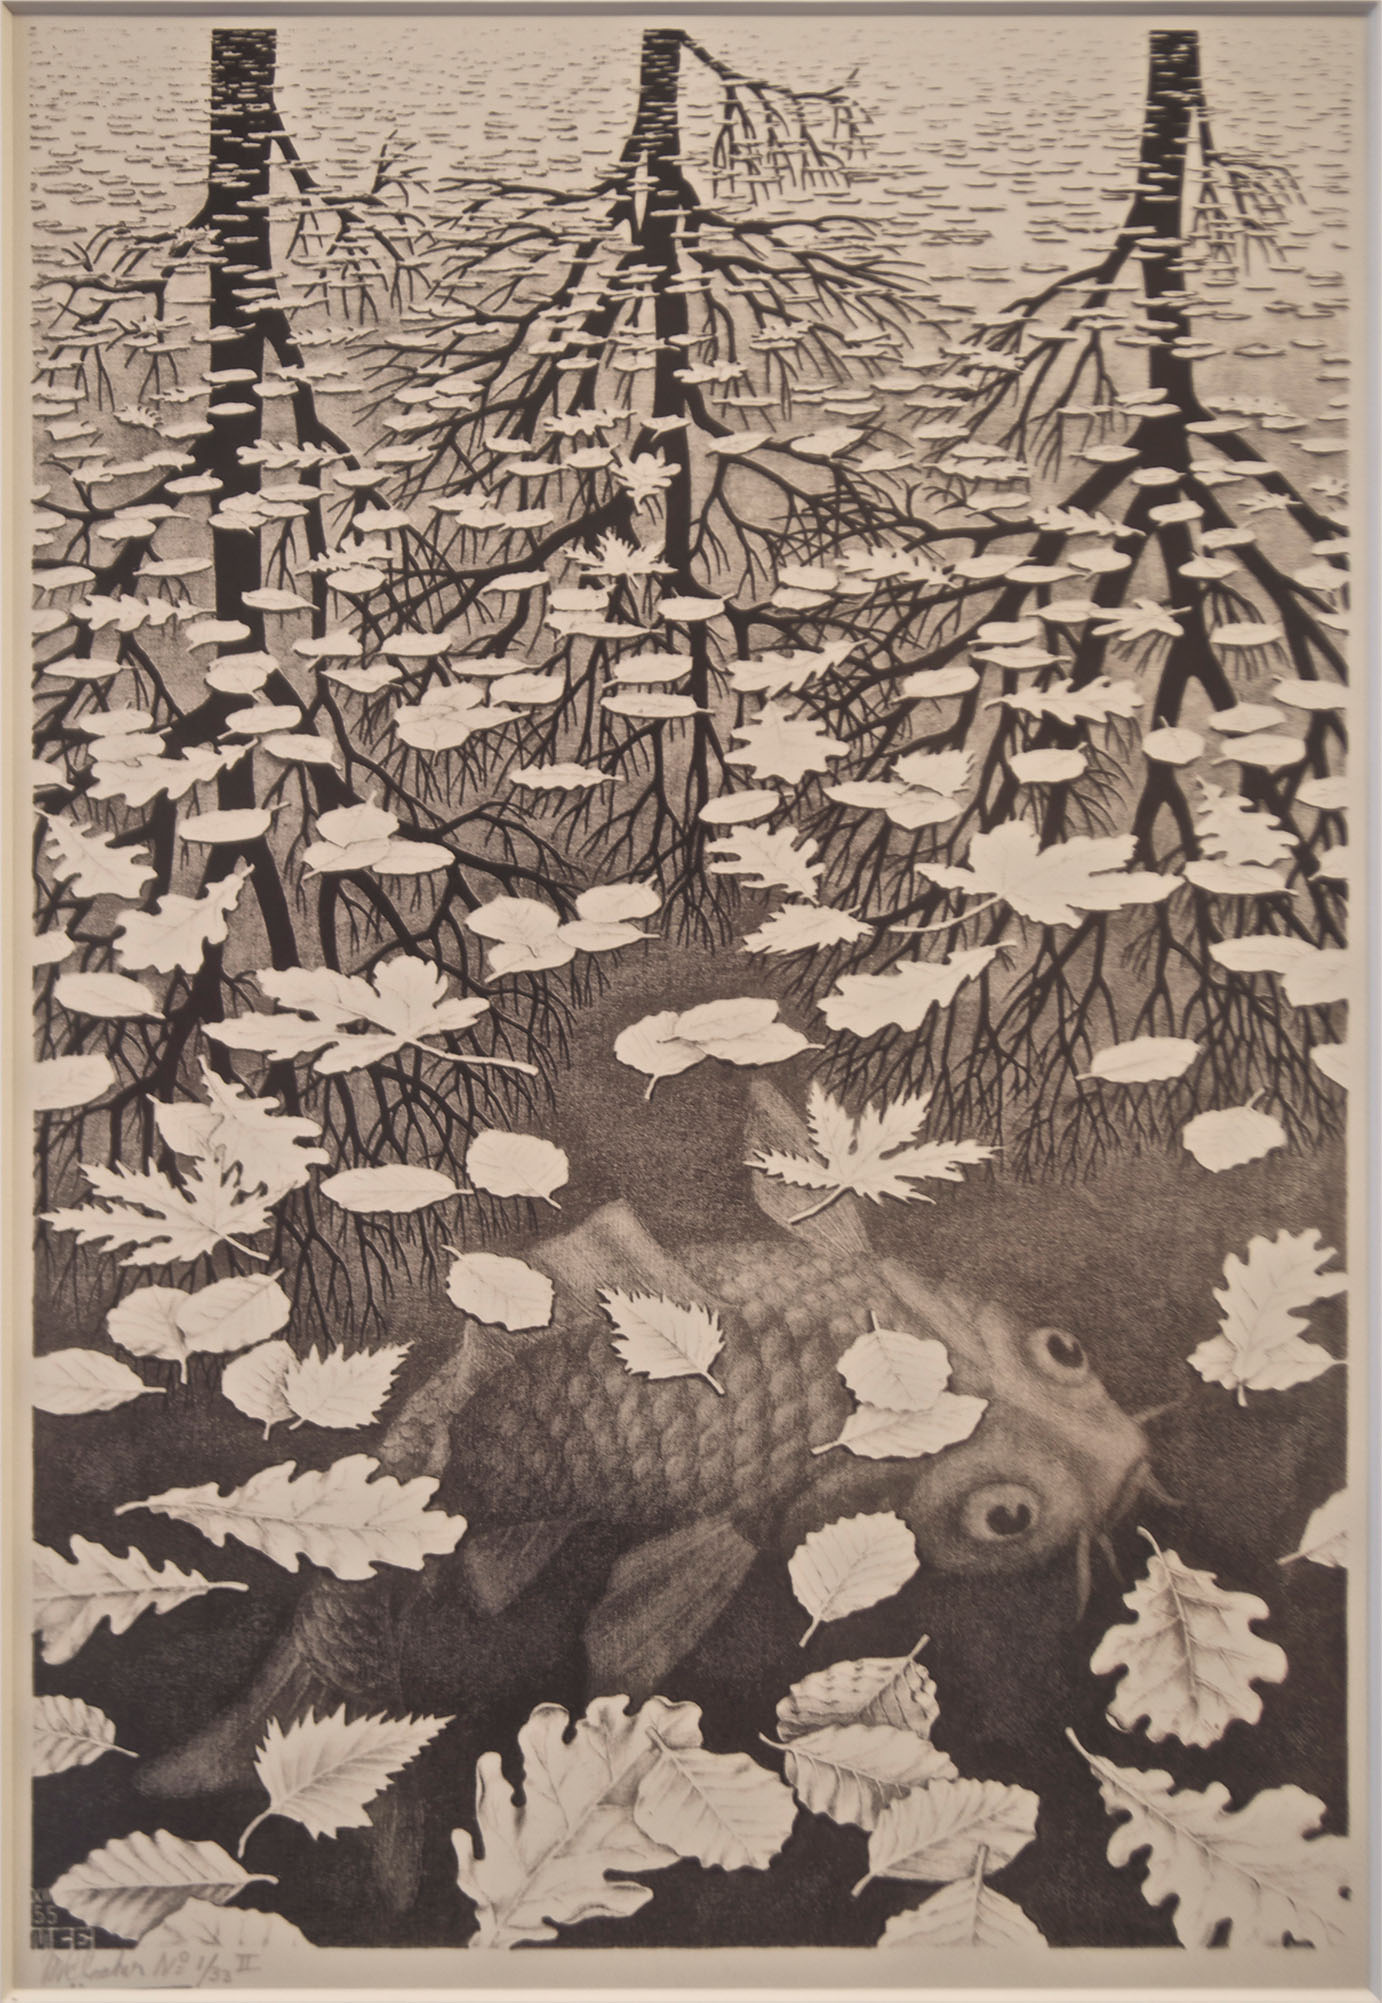
\includegraphics[height=.9\textheight]{img_046.jpg}
\caption[三界,艾舍尔作。]
  {三界,艾舍尔作(版画,1955)}
\end{figure}

不过,我们可以从不止一个层次来理解无门的评注。比如,考虑下面这个例子:\note{李普士书,第111--112页。中译文出自《禅宗无门关》。}

\begin{zenkoan}
公案:
南泉和尚问云:“还有不与人说的法么?”
泉云:“有。”
僧云:“如何是不与人说的法?”
泉云:“不是心,不是佛,不是物!”
无门曰:
\begin{zenkoan}
南泉被者一问,直得揣尽家私,郎当不少!
\end{zenkoan}
颂曰:
\begin{zenkoan}
叮咛损君德,无言真有功。
任从沧海变,终不为君通!
\end{zenkoan}
\end{zenkoan}

这首诗里,无门似乎说了些禅宗里非常核心的东西,而非一些傻话。然而奇怪的是,这首诗是自指的,因此它不仅评论了南泉所说的话,也阐明了自身的无效性。这种悖论是禅宗的一大特点。它是“破坏逻辑头脑”的一种尝试。从公案中同样也能看到这种悖论特质。看了无门的评注之后,你觉得南泉真的那么肯定他给的回答吗?或者他的回答的正确性根本就是无关紧要的?或者正确性这种东西在禅宗里就没有位置?正确性与真理之间的区别在哪里?或许这种区别是不存在的?如果南泉说“没有不与人说的法”,这又如何呢?结果会有什么不同吗?他的话还会记录在公案里而流传下来吗?

\begin{figure}
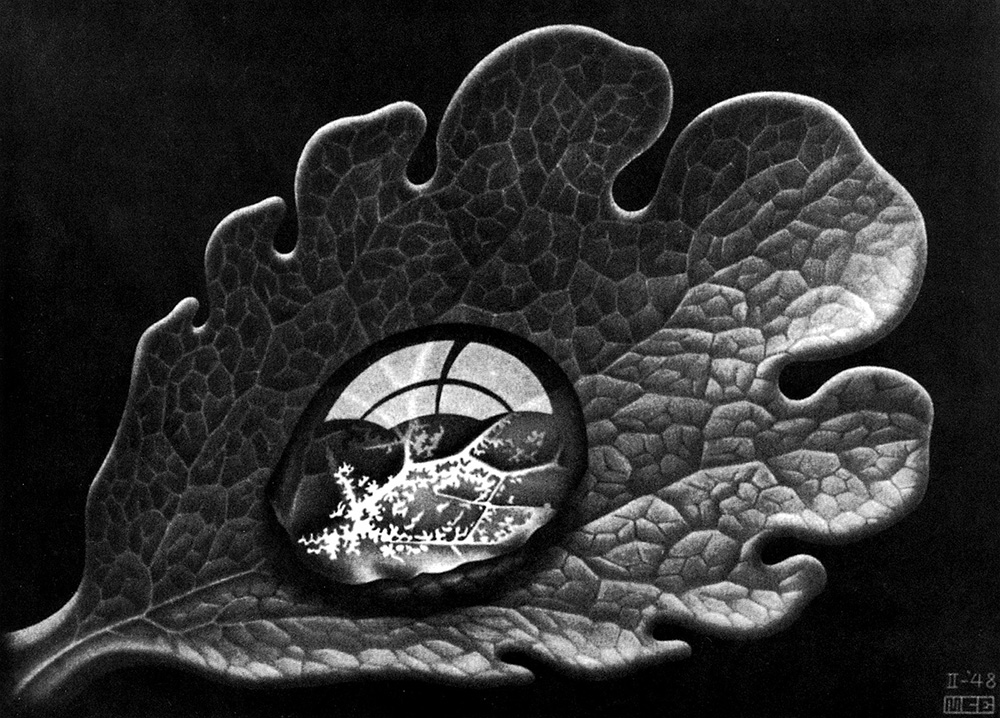
\includegraphics{img_047.jpg}
\caption[露珠,艾舍尔作。]
  {露珠,艾舍尔作(镂刻凹版,1947)。}
\end{figure}

这里是另一个旨在破坏逻辑头脑的公案:\note{《禅宗佛学》[\bn{Zen Buddhism}],纽约,Mout Vernon: Perter Pauper Press,1959年版,第22页。未查到原文,中文为译者所拟。有大方之家,望不吝赐教。}

\begin{zenkoan}
道悟趋禅师问曰:“吾欲求真理,吾应修至何等心境方可求之?”
师曰:“本来无心,故无心境可修;本来无真理,故无由求之。”
“既无心可修,无真可求,聚这些和尚此处习禅修行何故?”
师曰:“此处并无寸地,这些和尚何以聚得?吾口中无舌,何以集而教之?”
道悟问:“师何以言谎?”
师曰:“吾既无舌语人,何能言谎?”
道悟惘然曰:“吾不了师言。”
师曰:“吾亦不自了。”
\end{zenkoan}

如果有什么公案使人困惑,这就是一个。而且很可能它的目的恰恰就在于引起困惑,因为人的心智处于困惑状态时就会在某种程度上不合逻辑地运转。只有跨出逻辑,摆脱理论,人才能跃入顿悟境地。可是逻辑到底怎么不好了?为什么它会阻止人们达到顿悟?

\begin{figure}
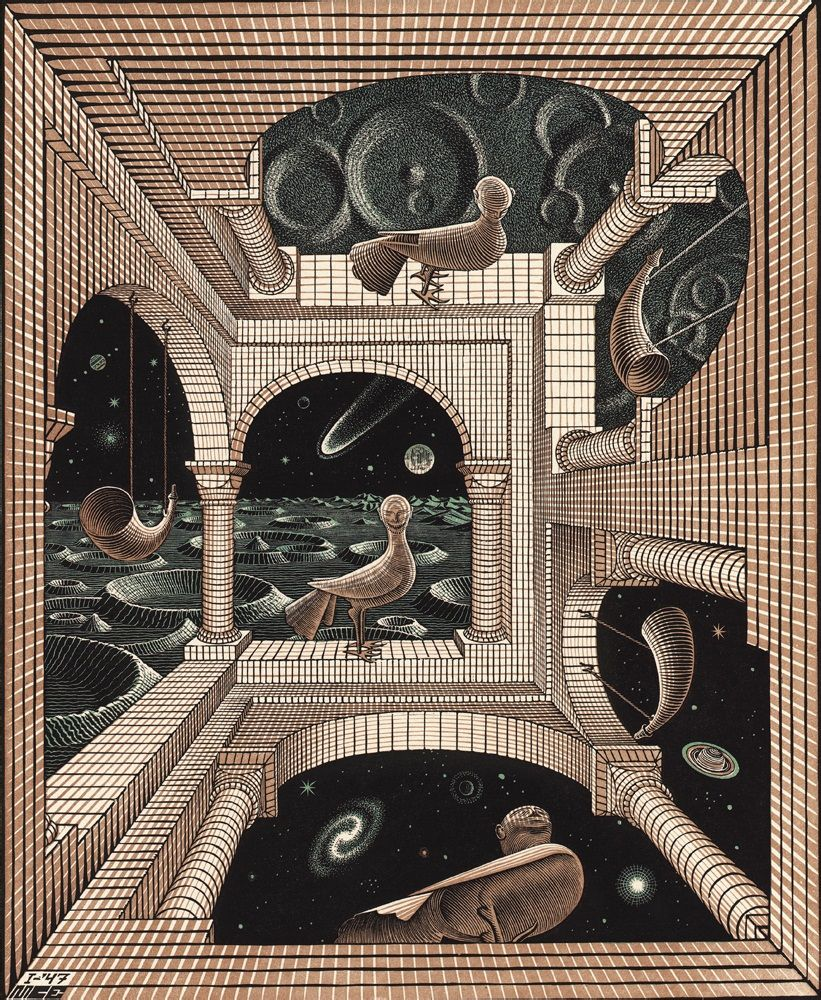
\includegraphics{img_048.jpg}
\caption[另一个世界,艾舍尔作。]
  {另—个世界,艾舍尔作(木雕版,1947)。}
\end{figure}

\section{禅宗反对二元论的斗争}

回答这些问题需要对顿悟是什么有一定的了解。所谓顿悟,最简明扼要地说或许就是:超越二元论。那么二元论又是什么呢?二元论就是把世界从概念上分划为种种范畴。这么一种非常自然的倾向能否被超越?我在“分划”前面加了一个修饰语“从概念上”,可能会让人觉得这是种智力上的或意识中的努力,因而也许会给人一种印象:克服二元论只需简单地抑制思维即可(好像抑制思维实际上很简单似的!)。但把世界裂成各种范畴也发生在远远低于思维这种较高层次的低层次上。事实上,二元论不仅是概念上对世界的划分,同样也是感知觉上对世界的划分。换句话说就是,人类的感知觉本质上是种二元现象——这使得追求顿悟至少是种逆水行舟般的奋斗了。

在禅宗看来,二元论的核心就是词语——普通的词。对词的使用必然导致二元化,因为每个词很明显地就是代表了一个概念范畴。所以,禅宗的一个主要部分就是为反对依靠词语而斗争。反对使用词语的最有力的工具之一就是公案,其中词被如此彻底地误用,以至那些认真看待公案的人会晕头转向,理不清自己的神智。因此,说顿悟的敌人是逻辑也许是不对的,它应该是二元化,借助词语的思维。事实上还要更基本:是知觉。一旦你感知到一个客体,你就把它与世界的其余部分划分开了;你人为地把世界分成部分,你于是就远离了“道”。

下面这个公案展示了同词语的斗争:\note{李普士书,第124页。中译文见《无门关》。}

\begin{zenkoan}
公案:
首山和尚拈竹篦示众云:“汝等汝人,若唤作竹篦则触;不唤作竹篦则背。汝诸人且道:唤作什么?”
无门曰:
\begin{zenkoan}
唤作竹篦则触;不唤作竹篦则背。不得有语,不得无语。速道,速道!
\end{zenkoan}
颂曰:
\begin{zenkoan}
拈起竹篦,行杀活令。
背触交驰,佛祖乞命!
\end{zenkoan}
\end{zenkoan}
\lnote{(这里的“佛祖”指的是禅宗的六位倍受尊崇的创建者,其中菩提达摩是初祖,慧能是六祖。)}

\begin{figure}
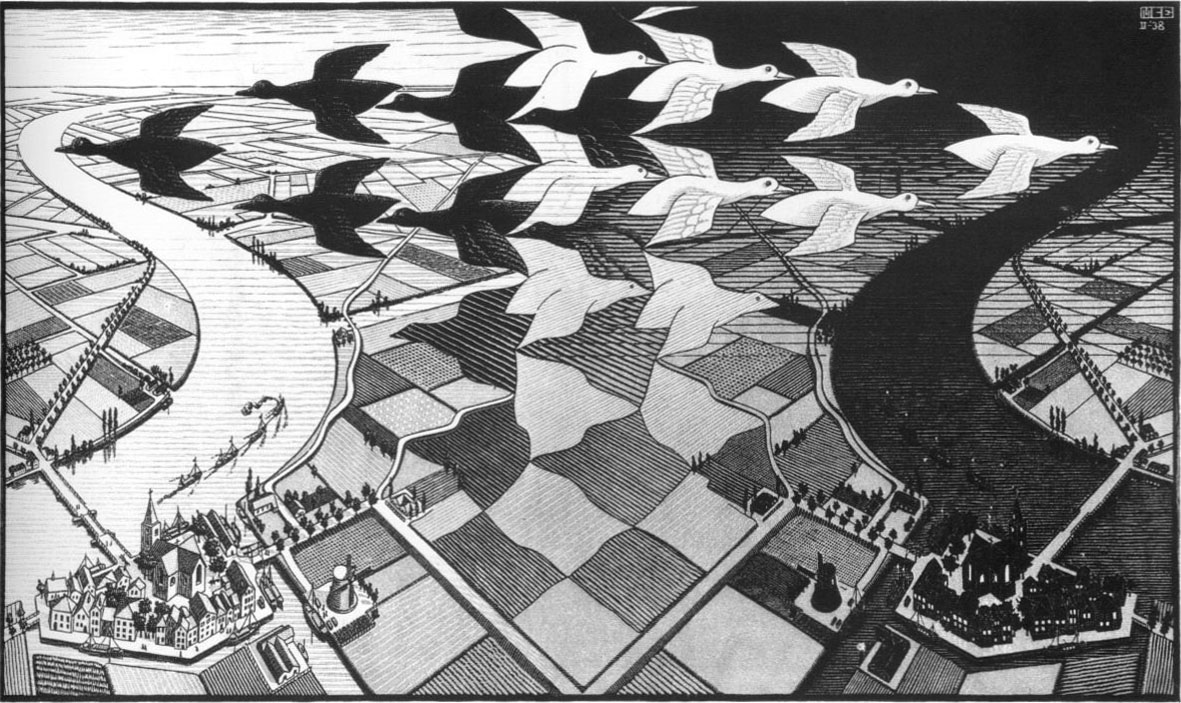
\includegraphics{img_049.jpg}
\caption[白天与黑夜,艾舍尔作。]
  {白天与黑夜,艾舍尔作(木刻,1938)。}
\end{figure}

为什么称之为竹篦就违反了它的实在性?可能是因为这种划类显得像是捕获了实在,而实际上这样的陈述却根本连表面都未能触及。可以比较一下“$5$是个素数”这个说法。那么多东西——无数多的事实依据——都省略掉了。另一方面,不称之为竹篦,那也的确是在无视一个特定的事实,不管这个事实是多么微不足道。因此,词语把我们引向某些真理——或许,同样也引向某些虚假——但肯定不能引向所有真理。你若是依赖词语走向真理,那就如同依赖一个不完全的形式系统而走向真理。一个形式系统的确会给你一些真理,但正如我们马上就会看到的,无论一个形式系统多么强有力,都不可能给出所有真理。数学家们的困窘就在于:除了形式系统,还有什么可以依靠?而禅宗信徒的困窘则是:除了词语,还有什么可以依靠?无门把这一困境阐述得很清楚:“不得有语,不得无语。”

下面又是南泉了:\note{《禅宗佛学》,第38页。中译文出自《无门关》。}

\begin{zenkoan}
公案:
南泉因赵州问:“如何是道?”
泉云:“平常心是道。”
州云:“还可趣向否?”
泉云:“拟向即乖!”
州云:“不拟怎知是道?”
泉云:“道不属知,不属不知;知是妄觉,不知是无记。若真达不疑之道,犹如太虚廓然洞豁,岂可说是非耶!”\lnote{[见\fig{50}]}
\end{zenkoan}

\begin{figure}
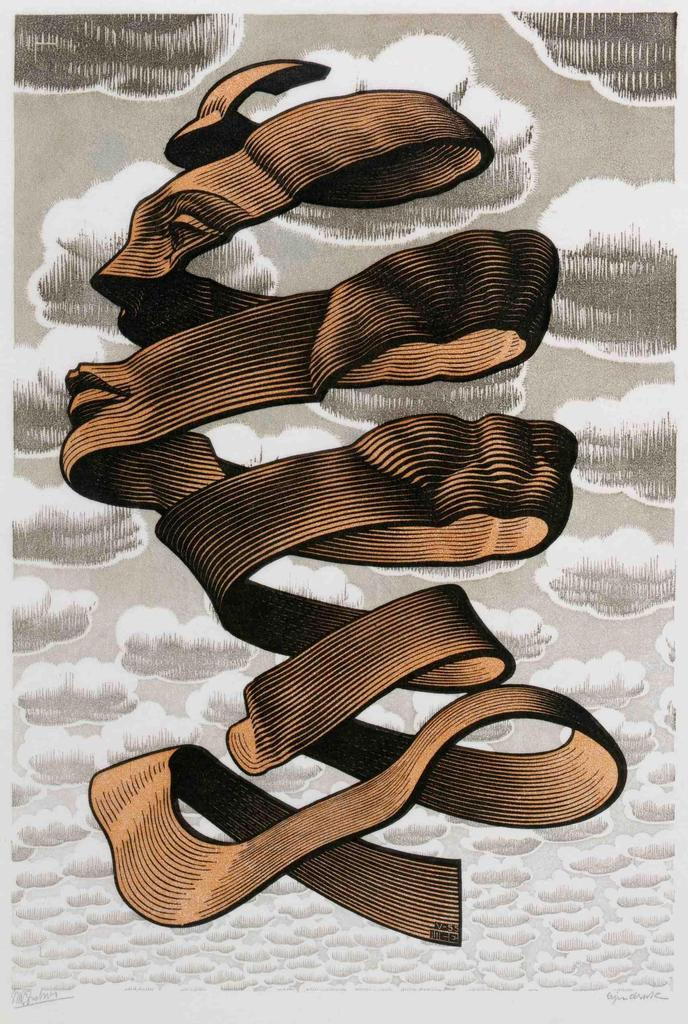
\includegraphics[height=.9\textheight]{img_050.jpg}
\caption[果皮,艾舍尔作。]
  {果皮,艾舍尔作(木雕,1955)。}
\end{figure}

这个奇特的陈述似乎充满了悖论。这多少让人想起那个治嗝偏方:“绕着大树跑三圈,脑子里始终不想‘乌鸦’这个词。”禅宗哲学似乎体现了这样一个观念:通向终极真理之路,就像那个唯一的治嗝偏方一样,会是充斥悖论的。

\section{主义、无方式以及云门}

如果词语不好,思维也不好,那么什么是好的?当然,这么问已经是彻头彻尾的二元论了,但我们是在讨论禅宗,无需假装出笃信禅宗的样子——因此我们可以试着来认真地回答这个问题。对于禅宗所追求的东西,我这里有个名称:“主义”。主义是反哲学的,是一神摒弃思维的存在方式。主义的大师是石头,树,蛤蟆。高等动物若想达到主义,就得经过一番奋斗,而且是永远不可能完全达到的。不过,人们偶尔还是会有幸瞥一眼主义的。也许下面这个公案就赐予了这么一瞥:\note{李普士书,第121页。中译文出自《无门关》。}

\begin{zenkoan}
公案:
沩山和尚始在百丈会中充典座,百丈将选大沩主人,乃请同首座对众下语,出格者可往。百丈遂拈净瓶置地上,设问云:“不得唤作净瓶,汝唤作什么?”
首座乃云:“不可唤作也。”
百丈却问于山,山乃倒净瓶而去。
百丈笑云:“第一座输却山子也!”因命沩为开山。
\end{zenkoan}

摒弃感知,摒弃逻辑、词语、二元化的思维——这就是禅宗的实质,主义的实质。这即是“无”方式——非智能,非机械,就是“无”。赵州处于无方式中,而这就是为什么他的“无”废问了那个问题。对于云门禅师,无方式是再自然不过的了:\note{吉奥麦·库伯斯[Gyomay M.Kubose],《禅宗公案》,第35页。中译文出自《五灯会元》下册,第九三二页。}

\begin{zenkoan}
\lnote{(云门禅师)}上堂,拈拄杖曰:“拄杖子化为龙,吞却乾坤了也。山河大地,甚处得来?”
禅宗采纳整体论,并且推向逻辑上的极端。如果整体论是断言事物必须作为一个整体被理解,而非其各个部分的总和,那么禅宗走得更远,认为整个世界根本就不能被划分为一个个事物。划分世界就会误入岐途,因而就不能达到顿悟了。
公案:\note{《禅宗佛学》第31页。不知出处,中译文为译者自拟。}
一师因一僧问曰:“如何是道?”
师曰:“正眼前是道。”
“如何我不自见?”
“汝自虑故。”
“师知之否?”
师曰:“汝但见二分:言‘我不自见’,、‘师见之’,汝目障矣。”
\begin{zenkoan}
“无我无你,可得见否?”
“无我无你,谁欲见之?”
\end{zenkoan}
\end{zenkoan}

很明显,禅师想传达这样一种观念,即顿悟状态意味着自我和宇宙之间的分界消解了。这将是二元论的真正终结,因为正如他所说的,任何一个有感知愿望的系统都将不复存在。但除了死亡,那还能是种什么状态?一个活生生的人怎么能消解他自己与外部世界之间的分界线呢?

\section{禅宗与堕界}

禅宗和尚拔对给一个行将圆寂的门人写了一封信,信中说:“汝之无终之终,一似雪片溶于清气之中。”雪片,曾是宇宙中完全可见的一个子系统,现在溶解于它曾依托的那个更大的系统中了。虽然它已不再是以一个清晰可见的子系统而存在,其实质却依然是存在的,并将这么保持下去。它漂浮在堕界中,与没打出的嗝在一起,与没人读的故事中的人物在一起……这是我对那番话的理解。

禅宗认识到了自身的局限,正如数学家们逐渐也认识到了公理化方法作为获得真理的方法其局限所在。这并不意味着禅宗对自身之外有什么东西有个确切的答案。数学家们不清楚在形式化推理之外还有什么有效的推理形式,禅宗也强不了多少。关于禅宗的界限,下面这个奇怪的公案给了一个清楚的禅宗说法,看上去很能代表南泉的精神:\note{库伯斯书,第110页。中译文出自《五灯会元》,中册,第七八二页。}

\begin{zenkoan}
师\lnote{(洞山禅师——译注)}谓众曰:“知有佛向上人,方有语话分。”
僧问:“如何是佛向上人?”
师曰:“非佛。”
\end{zenkoan}

总是能走得更远。顿悟并非禅宗的终点。而且并没有一付超越禅宗的良方。唯一坚实可靠的是,佛非道也。禅宗是一个系统,不可能成为它自己的元系统。总是有东西处在禅宗之外,那是无法在禅宗之内完全了解或说清楚的。

\section{艾舍尔与禅宗}

在质疑感知、设置无答案的荒唐哑谜方面,禅宗有个伴儿:画家艾舍尔。比如《白天与黑夜》(\fig{49})这幅“背触交驰”(借用无门的话)的杰作。人们会问,“那些真的是鸟吗?那些真的是田野吗?那真的是白天吗?真的是黑夜吗?”然而我们又都知道这么问毫无意义。这幅画同禅宗的公案一样,是在努力打破逻辑头脑。艾舍尔还特别喜欢作一些矛盾的画,像《另一个世界》(\fig{48})——把实在与非实在摆弄来摆弄去,与禅宗摆弄实在与非实在的方式完全一样。是否应该认真对待艾舍尔?是否应该认真对待禅宗?

在《露珠》(\fig{47})中,对于反射有种精致的、俳句般的探究。另外还有两幅月亮映在平和的水面上的宁静图景:《泥塘》(\fig{51})和《水面涟漪》(\fig{52})。水中的月亮是许多公案的主题。下面是一个例子:\note{库伯斯书,第120页。这是一个日本公案,中译文采自《禅的故事》(即李普士《禅肉,禅骨》一书的中译本),哈尔滨:北方文艺出版社,1987年版。}

\begin{zenkoan}
千代能尼师在园觉佛光大师会下学禅,久久不能获得参悟的结果。一个月明之夜,千代以一个旧桶提水,偶因桶箍破裂而桶底脱落,豁然获得大自在,作一偈以记其事:
\begin{zenkoan}
扶持旧桶,桶底忽脱。
桶里无水,水中无月。
\end{zenkoan}
\end{zenkoan}

《三界》是一幅艾舍尔的画(\fig{46}),也是一个禅宗公案的主题:\note{库伯斯书,第180页。中译文出自《五灯会元》,中册,第三七八页。}

\begin{zenkoan}
\lnote{(瑞岩)}问:“三界竞起时如何?”
师\lnote{(岩头禅师)}曰:“坐却著。”
曰:“未审师意如何?”
师曰:“移取庐山来,即向汝道。”
\end{zenkoan}

\begin{figure}
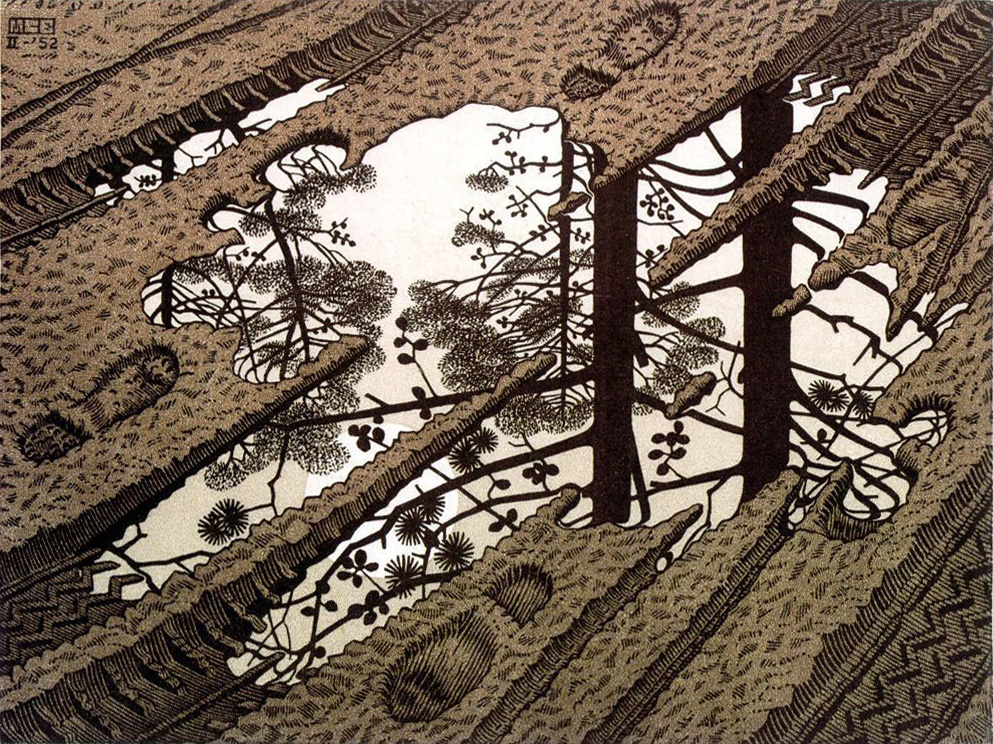
\includegraphics{img_051.jpg}
\caption[泥塘,艾舍尔作。]
  {泥塘,艾舍尔作(木刻,1952)。}
\end{figure}

\section{“三比二”与艾舍尔}

在《辞》(\fig{149})里,相左的事物在不同的层次上被纳入了一个统一体。顺着这幅画我们看到逐渐的变迁:从黑鸟到白鸟到黑鱼到白鱼到黑蛙到白蛙到黑鸟……六步之后,回到了我们开始的地方!这是调和黑与白这两分,还是鸟、鱼、蛙这三分?或者是$2$的偶数性与$3$的奇数性之间的对立导致的六位一体?在音乐里,六个等长音符会造成节奏岐义——是两个一组的三组,还是三个一组的两组?这种岐义有个名称:“三比二”。肖邦是“三比二”的大师:见他的华尔兹(作品42号)、练习曲(作品25号之二)。在巴赫的作品中,出现了这种现象的有第五键盘组曲中的小步舞曲,以及那首不可思议的G小调第一无伴奏小提琴奏鸣曲的终曲。

\begin{figure}
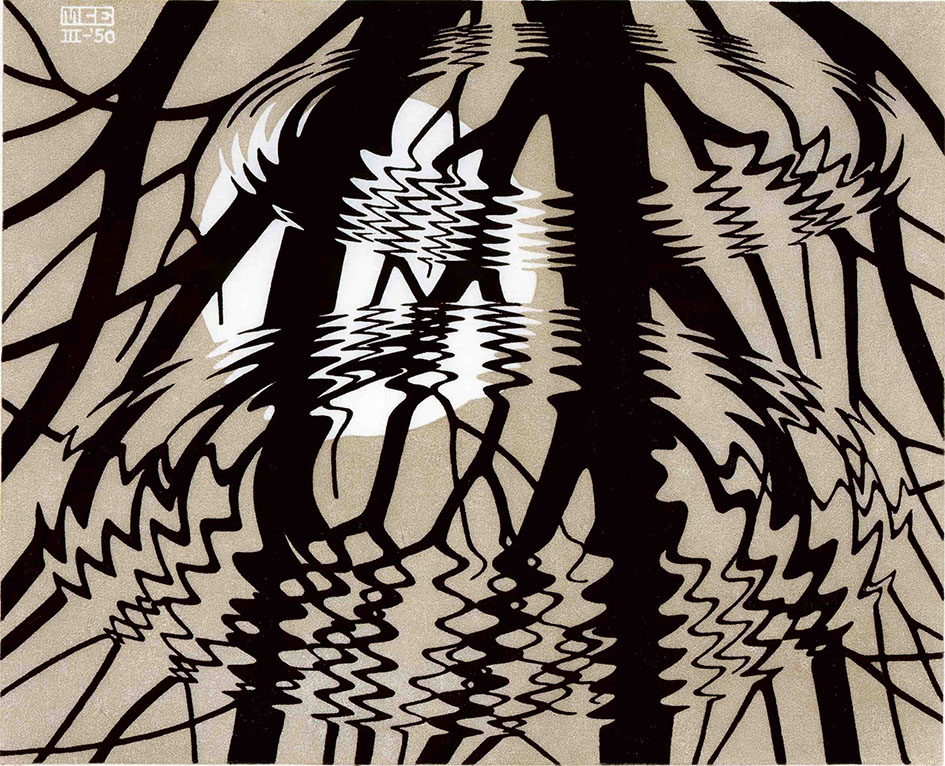
\includegraphics{img_052.jpg}
\caption[水面涟漪,艾舍尔作。]
  {水面涟漪,艾舍尔作(油毡浮雕,1950)。}
\end{figure}

逐步进入到《辞》的中央时,差别便渐渐开始模糊。于是到最后剩下的不是三个,也不是两个,而是一个单质:“辞”(画中是拉丁文VERBUM,就是“辞”的意思)在熠熠闪光——也许这就是顿悟的象征。有趣的是,“辞”不仅是个词,而且它的意义也即“词”——并不完全与禅宗的观念相符。另一方面,“辞”是画中唯一的一个词。洞山禅师曾说过,“全部佛经三藏可以由一个字来表达。”我一直在想,该是什么样的解码机制才能从一个字里抽出三藏经文?也许是个带有两个半球的东西。

\section{因陀罗之网}

\begin{figure}
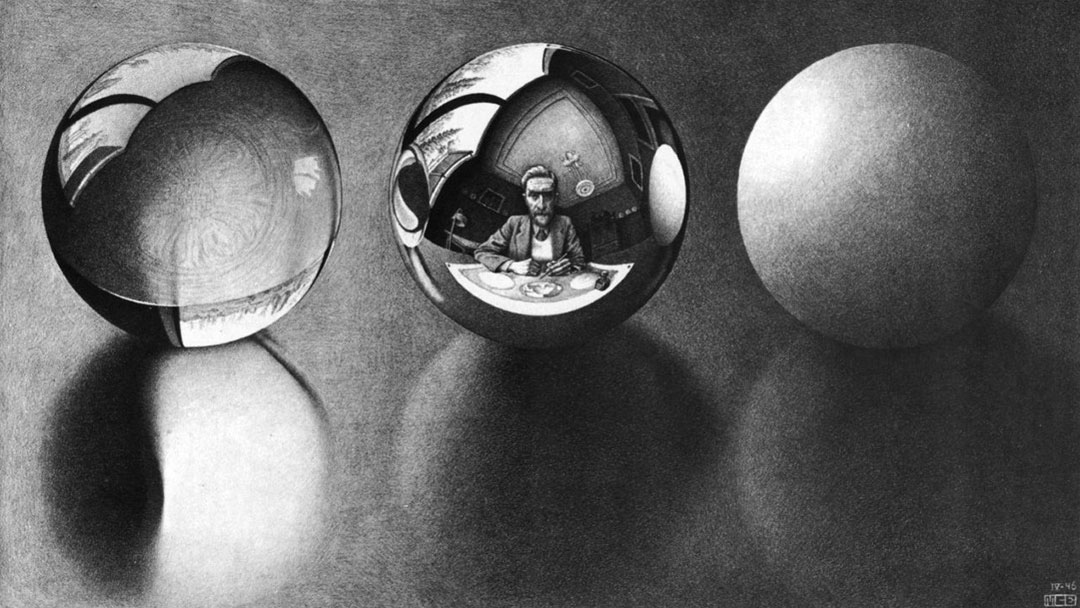
\includegraphics{img_053.jpg}
\caption[三个球II,艾舍尔作。]
  {三个球II,艾舍尔作(版画,1946)。}
\end{figure}

最后,我们来看看《三个球之二》(\fig{53}),其中世界的每个部分都包含了、同时也被包含于其它部分:写字台反映出在它上面的球,球与球之间彼此反映,同时也反映出写字台,并反映出这幅画本身以及正在作画的艺术家。所有的事物彼此之间都有着无尽的联结。这里还只不过是给个提示,然而提示已经足够了。佛教中的因陀罗之网就象征着遍布宇宙的一张无穷无尽的线网,水平的线穿过空间,垂直的线穿过时间。每个线与线的交汇处都是一个个体,每个个体都是颗明珠。“神”的巨大光芒照耀并穿透每颗明珠,而且,每颗明珠不但在反映网上其它明球的光泽——也反映着遍布于宇宙的每一反映的每一反映。

这使我脑子里产生了一幅重正化粒子的图像:在每个电子中,都有虚光子、正电子、中微子、$\uppi$介子……;每个光子中又有虚电子、质子、中子、$\uppi$介子……;而在每个$\uppi$介子中,有……

但随即又来了另一幅图像:关于人。每个人都反映在许多其他人的脑子里,那些人又反映在另外一些人的脑子里,如此下去。

这两幅图像都能由扩充迁移网简明漂亮地表示出来。在粒子的情形,将是每个粒子范畴都有一个网;在人的情形,是每个人有个网。每个网都含有对其它网的调用,这样就在每个ATN周围包上了一个ATN的虚云。调用某一个网导致对别的网的调用,这个过程在终了之前会像多级瀑布般地流泻到任意远。

\section{无门论无}

让我们回到无门,把这番闲扯收归于禅宗。下面是他对赵州的“无”的评论:\note{李普士书,第89--90页。中译文出自《无门关》。}

\begin{zenkoan}
参禅须透祖师关,妙语要穷心路决。祖关不透,尽是依草附木精灵。且道:如何是祖师关?只者一个“无”字,乃宗门一关也。遂目之曰:“禅宗无门关。”透得过者,非但亲见赵州,便可与历代祖师把手共行,眉毛厮结,同一眼见,同一耳闻,岂不庆快?莫有要透关底么?将三百六十骨节、八万四千毫窍,通身起个疑团,参个“无”字,昼夜提撕。莫作虚无会,莫作有无会,如吞了个热铁丸相似,吐又吐不出,荡尽从前恶知恶觉;久久纯熟,自然内外打成一片,如哑子得梦只许自知;蓦然打发,惊天动地,如夺得关将军大刀入手,逢佛杀佛,逢祖杀祖,于生死岸得大自在,向六道四生中游戏三昧。且作么生提撕?尽平生气力举个“无”字。若不间断,好似法烛,一点便着。
\end{zenkoan}

\section{从无门到"WU"谜题}

我们现在从赵州的“无”那无比漂渺的高度上降下来,降到单调又平凡的侯世达的"WU"……我知道你已为这个"WU"花费了不少精力(读第一章的时候),所以我现在很愿意摆出答案了。那时提出的问题是:

\begin{block}
“"WU"还有定理性也无?”
\end{block}

答案并非一个含糊其词的“无”,而是一声响亮的“不”。为了指明这一点,我将借用二元论的、逻辑的思维。

在第一章中有两点观察是至关重要的:

\begin{enumerate}
\item "WU"谜题之所以有难度,很大程度上是因为它涉及了加长规则与缩短规则两者的交织;
\item 解开这个谜题的希望还是有的,只是要借助一个工具:数论。某种意义上讲,数论在处理这种复杂度的问题时具有合适的深度。
\end{enumerate}

第一章里我们没有非常仔细地从这种角度来分析"WU"谜题,现在我们就要这么做了。我们会见到那第二点观察(当推广一下,超出意义不大的"WJU"系统的时候)是数学界最富成果的发现之一,它改变了数学家们对自己那门学问的看法。

为使读者参考起来方便,我重述"WJU"系统如下:
\begin{rulelist}
\item[符号]"W","J","U"
\item[公理]"WJ"
\item[规则]
\begin{enumerate}[labelindent=0pt, label=\Roman*.,
  format=\sffamily\bfseries, before*=\FixItemIndent]
\item 若$x"J"$是定理,则$x"JU"$也是定理。
\item 若$"W"x$是定理,则$"W"xx$也是定理。若$"W"x$是定理,则$"W"xx$也是定理。
\item 在任何定理中,"JJJ"可以被换成"U"。
\item "UU"可以从任何定理中删去。
\end{enumerate}
\end{rulelist}

\section{无门告诉我们如何解开"WU"谜题}

于是,按照上述两点观察,"WU"谜题无非是一道披着印符外衣的自然数问题。假若我们能想出一个办法,把它转换到数的领域里,我们大概就能解它了。让我们好好想想无门的话:“若向者里着得一只眼,便知清凉国师败阙处。”但“着得一只眼”又怎样呢?

你要是数一数定理中"J"的数目,很快你就会发现好像永远不会是$0$。换句话说,似乎无论折腾多少回加长与缩短的操作,我们永远也得不到一个清除了所有"J"的符号串。让我们把串中J的数目称作该串的“眼”数,因为"J"的存在就好像是在我们想要的"WU"串中间钻了一些“洞眼”。注意公理"WJ"中有一只“眼”。我们不但可以说明定理的“眼”数不可能是$0$,还可以说明,“眼”数永远不会是$3$的倍数。

作为开始,先注意规则I与规则IV对“眼”数丝毫不发生影响。所以我们只需要考虑规则II与III。规则III只不过是使“眼”数恰好减$3$,使用这个规则之后,得到的输出或许也可能是$3$的倍数——但仅只在输入已经是$3$的倍数这一情况下。简而言之,规则III决不会无中生有地产生$3$的倍数。它必须在“眼”数已经是$3$的倍数的情况下才能产生“眼”数为$3$的倍数的串。同样的事情也发生在规则II身上,因为它使“眼”数翻倍。理由是,若$2n$被$3$整除,那么——由于$3$不整除$2$——$n$就得被$3$整除(数论里的一个简单事实)。无论是规则II还是规则III,都不能无中生有地产生$3$的倍数。

而这恰恰就是解开"WU"谜题的关键所在!下面是我们已经知道了的事情:
\begin{enumerate}
\item  最一开始的“眼”数是$1$(不是$3$的倍数);
\item 有两条规则丝毫不影响“眼”数;
\item 另两条规则的确要影响“眼”数的值,但除非初始给出的是$3$的倍数,否则它俩也决不会产生$3$的倍数。
\end{enumerate}

结论是——也是典型的继承性论证方式——“眼”数永远无法变成$3$的倍数。特别地,$0$就决不可能是“眼”数的值了。因此,"WU"不是"WJU"系统的定理。

请注意,即使是作为一个关于“眼”数的谜题,这个问题也会因为加长规则与缩短规则的交织而使人迷惑。零成了追求目标,

“眼”数可以增大(规则II),可以减小(规则III)。我们大概会想,不断地换着使用那些规则,最终或许能达到$0$,于是就这么干了下去,直到我们站出来分析一番我们面临的到底是什么。现在,多亏一个简单的数论推理过程,我们知道了那是不可能的。

\section{对"WJU"系统进行哥德尔配数}

并非所有以"WU"谜题为代表的那类问题都像"WU"谜题那么容易解。但我们已经看到了至少有这么一个这种问题是可以嵌入数论并用数论来解决的。我们现在就要看到,有那么一种方法,可以把所有的关于任何形式系统的问题都嵌入数论。这之所以能做到是因为哥德尔所发现的一种特殊的同构。下面我用"WJU"系统来说明这种方法。

我们从"WJU"系统的记号开始。先把每个符号都映射到一个新的符号上去:
\[
\begin{array}{r>{\iff}cl}
"W" & & 3 \\
"J" & & 1 \\
"U" & & 0
\end{array}
\]

这个对应是任意选定的。若要一定说出个理由,可以说每个符号都多少有点像它所映上的那个新符号。每个数都称作相应字母的哥德尔数。现在我敢肯定你已经猜到了字母串的哥德尔数将是什么了:
\[
\begin{array}{r>{\iff}cl}
"WU"   & & 30 \\
"WJJU" & & 3110 \\
       &\multicolumn1c{\text{等等}}
\end{array}
\]

这很简单。很清楚,这个记号间的映射是个保持信息的变换,就像是在两个不同的乐器上演奏同一旋律。

我们现在来看看"WJU"系统中的一个典型的推导,我们同时用两种记号写:

\begin{longtabu}[c]{!{(\arabic{taburow})\quad}r!{——}c!{——}>{$}l<{$}}
"WJ"      & 公理     & 31 \\
"WJJ"     & 规则2 & 311 \\
"WJJJ"    & 规则2 & 31111 \\
"WUJ"     & 规则3 & 301 \\
"WUJU"    & 规则1 & 3010 \\
"WUJUUJU" & 规则2 & 3010010 \\
"WUJJU"   & 规则4 & 30110
\end{longtabu}

左边一列是使用我们已熟悉的四条印符规则而得到的。右边一列同样也可以当作是使用了一组类似的印符规则而生成的。不过右边的一列有种二重性。下面我来解释。

\section{从印符和算术两个角度看问题}

我们可以说第五个串(“$3010$”)是从第四个来的,方法是在右边放上一个“$0$”;另一方面,我们同样也可以把这一转换看成是由于算术运算而导致的——确切地说就是乘以$10$。当自然数按十进制写出时,乘以$10$和在右边放上一个$0$是没有差别的。我们可以利用这一点写出一条算术规则,与印符规则I相对应:
\begin{thm}{算术规则Ia}
一个数的十进制展开的右侧如果以$1$结尾,则可乘以$10$。
\end{thm}

我们可以不必指称十进制展开中的符号,而用算术方式来描述最右边的数字:
\begin{thm}{算术规则Ib}
一个数被$10$除时的余数如果是$1$,则可乘以$10$。
\end{thm}

我们可以仍是固守纯粹的印符规则格式,比如下面这个:
\begin{thm}{印符规则I}
从任何一个最右侧符号为“$1$”的定理都可以得到一个新的定理,方法是在那个“$1$”右侧拼上一个“$0$”。
\end{thm}
它们的效果是一样的。这就是为什么右边一列具有“二重性”:可以视为一系列的印符操作,改变着符号排列模式;也可以视为一系列算术运算,改变着数的量级。但有充足有力的理由使我们对算术的版本更感兴趣。跨出一个纯印符系统,再走入另一个同构的印符系统,这没有多大意思;而离开印符领域然后步入一个与之同构的数论的某个部分则会激发出未开发的潜力。这就像一个人前半生一直通晓乐谱,但只是用眼睛看而已——然后,忽然有一天,有人告诉了他声音与乐谱之间的映射。那将是怎样一个崭新而又丰富的世界!在这里,就好像一个人前半生一直都熟知符号串的样子,但只是那些串的形状而已,从不知意义何在——然后,忽然有一天,有人告诉了他事物与串之间的映射。这是怎样的一种启迪!哥德尔配数的发现被人们比作笛卡尔关于平面曲线与二元方程之间同构的那个发现:一旦你见到了,真是令人难以置信地简单——而一个崭新宽广的世界就这么展开了。

不过,在我们跳到结论之前,你或许会愿意看看这个同构的较高层次的全貌是什么样。这也是个很好的练习。其思想在于使给出的各个算术规则与"WJU"系统的每个印符规则在效果上没有差别。

下面是实现的方案之一。规则中的$m$和$k$是任意的自然数,$n$是小于$10^m$的任何自然数。

\begin{thm}{规则1}
若有了$10m+1$,则还可以有$10\times(10m+1)$。

\emph{例子}:从第$4$行到第$5$行。这时,$m=30$。

\item[规则2]
若有了$3\times10^m+n$,则还可以有$10^m\times(3\times10^m+n)+n$。

\emph{例子}:从第1行到第2行,这时$m$与$n$都是$1$。

\item[规则3]
若有了$k\times10^{m+3}+111\times10^m+n$,则还可以有$k\times10^{m+1}+n$。

\emph{例子}:从第3行到第4行,这时$m$与$n$都是$1$,而$k$是$3$。

\item[规则4]
若有了$k\times10(m+2)+n$,则还可以有$k\times10(m)+n$。

\emph{例子}:从第6行到第7行。这时,$m=2$,$n=10$,$k=301$。
\end{thm}
可别忘了我们的公理!没有它我们哪里都去不了。所以,我们说:
\[
\text{我们有$31$。}
\]
现在,右边一列可被视为一个资格充分的算术过程了,它来自一个新的算术系统,不妨称之为$310$系统:

\begin{longtabu}[c]{!{(\arabic{taburow})\quad}>{$}r<{$}>{\quad}l}
31      & 给定的 \\
311     & 规则2($m=1$,$n=1$) \\
31111   & 规则3 \\
301     & 规则3 \\
3010    & 规则1($m=30$) \\
3010010 & 规则2($m=3$,$n=10$) \\
30110   & 规则4($m=2$,$n=10$,$k=301$)
\end{longtabu}

请看,加长与缩短规则还在追着我们,这个“$310$系统”也被缠上了。这个东西被传送到了数的领域,使得哥德尔数时而大时而小。如果细细观察,你会发现这些规则的设计是基于一个并不深奥的思想:整数的十进制表示中那些数码的左右移动是与乘以或除以$10$的方幂相关联的。这一简单的结论可以推广:

\begin{thm}{中心命题}
若有一条印符规则,它在任一十进制表示的数中移动、改变、删除或插入数码,那么这条规则可同样由一条算术规则来替代,后者包括对$10$的方幂的算术运算以及加、减等运算。
\end{thm}
简而言之:

\begin{block}
用于数字的印符规则实际上等同于用于数的算术规则。
\end{block}

这一简单的结论是哥德尔方法的核心,其后果是震撼人心的。就是说,一旦对一个形式系统进行了哥德尔配数,立刻就有了一组规则,使我们得到完整的哥德尔同构。结果就是,我们可以把对任一形式系统的研究——事实上即对所有形式系统的研究——转成数论工作。

\section{WJU可产生的数}

就像一组印符规则会产生一集定理,一集相应的自然数可通过重复使用算术规则而生成。这些可产生的数在数论中扮演的角色与形式系统中定理扮演的角色是一样的。当然,什么样的数是可产生的,这取决于采用的是什么规则。“可产生的”数的可产生性是相对于一个算术规则的系统而言的。例如,诸如$31$,$3010010$,$31111$等等这样的数可以称为“"WJU"可产生的”数——一个笨拙的词,或许该简称为“"WJU"数”,意指这些数是把"WJU"系统通过哥德尔配数转入数论的产物。假若我们是对"pq"系统进行了哥德尔配数,然后把其规则“算术化”,那么我们可以称那些可产生的数为“"pq"数”——如此等等。

注意,可产生的数(对任一给定了的系统)是由递归方法定义的:给定一些已知的可产生的数,我们的规则就告诉我们如何得到更多可产生的数。于是,可产生的数组成的类就是在不断地扩大,很像斐波那契数列或$\mQ$数的增长方式。任一形式系统的可产生的数构成的集合都是一个递归可枚举集合。其补集——不可产生的数构成的集合怎么样呢?也总是递归可枚举的吗?那些不可产生的数有没有什么共同的算术特征?

当你把形式系统研究换成数论研究时,就会产生这类问题。对每个算术化了的系统都可以问,“我们能否用一种递归可枚举的办法刻划不可产生的数?”这些都是数论中很困难的问题。对现在那些已经算术化了系统,这种问题都会显出是些极难解决的问题。不过,假如存在解决办法,那也必将是依靠通常那种用于自然数的一步一步的推理。而这当然也就是在我们前些章讲过的那种典范形式中进行的。TNT整个看来似乎抓住了所有有效的数学思维过程,并都压入一个紧凑的系统中了。

\section{咨询TNT以解答有关可产生的数的问题}

那么,是不是说有可能解答任何有关形式系统问题的方法都已经在这么一个形式系统——TNT——里面了呢?似乎这是可以想象的。比如看下面这个问题:

\begin{block}
"WU"是"WJU"系统中的定理吗?
\end{block}
找到答案等同于确定$30$是否是一个"WJU"数。由于这是一个数论陈述,我们该可以设想,经过一番艰苦工作就能想出办法把句子“$30$是一个"WJU"数”翻译成TNT记号,其过程与想出如何把其它数论句子翻译成TNT记号是差不多的。我该立刻提醒读者,这样的翻译确实存在,但极其复杂。你也许还记得,在第八章里我指出过:即使像“$b$是$10$的方幂”这么简单的算术谓词,要转成TNT记号的形式都是非常棘手的——而谓词“$b$是个"WJU"数”则还要复杂得多!可这还是能做到的。这个问题中的$b$可被数字
\[
SSSSSSSSSSSSSSSSSSSSSSSSSSSSSS0
\]
替换。得到的结果将是一个硕大无朋的TNT符号串,一个谈论WU谜题的TNT符号串。就让我们称之为“无朋”吧。通过无朋及与之类似的串,TNT现在可以“用码”来谈论"WJU"系统了。

\section{无朋的两重性}

为了从这个对原问题的奇特的转换中得到更多的好处,我们得寻找下面这个新问题的答案:

\begin{block}
无朋是TNT的定理吗?
\end{block}

我们做的只不过是把一个相对短小的串("WU")换成了另一个(硕大的无朋),把一个简单的形式系统("WJU"系统)换成了一个复杂的(TNT)。虽然把问题这么修饰了一番,解决并不见得容易些。实际上,TNT中的加长和缩短规则更多更全了,所以把问题这么改装一下很可能比原问题要难解决得多。甚至你可能会说通过无朋来看"WU"纯属故弄玄虚。不过,我们可以在不止一个层次上看待无朋。

事实上,这一点是很令人感兴趣的:无朋有两种不同的被动意义。首先,是我们已经给出了的:
\begin{center}
$30$是个"WJU"数。
\end{center}
其次,我们知道这个陈述与下述陈述有关联(通过同构):
\begin{center}
"WU"是"WJU"系统中的定理。
\end{center}
所以我们可以合法地引用后者作为无朋的第二个被动意义。这也许会显得有些奇怪,因为毕竟无朋只不过是由一些加号、括号等等TNT中的符号组成的东西。它怎么可能表达出没有算术内容的陈述呢?

事实是,它能。正如一串单音在一支曲子里既可以构成旋律也可以构成和声,正如“BACH”可以解释成名字也可以解释成旋律,正如单独一个句子可以同时是精确地从结构上描述艾舍尔的一幅画、DNA的一个节断、巴赫的一支曲子、嵌有这个句子的一个对话,无朋也可以从(至少)两个完全不同的角度来理解。发生这种事情是由于下述两个事实:
\begin{enumerate}[labelindent=0pt, label=事实\arabic*, format=\textsf]
\item 像“"WU"是个定理”这样的陈述可以通过哥德尔同构编码成一个数论问题。
\item 数论陈述可以翻译到TNT系统中去。
\end{enumerate}
可以说,有了事实1,无朋就是一则编了码的消息,有了事实2,用于该编码的符号就是TNT的符号。

\section{编码与隐含意义}

有一种观点认为,一则编了码的消息与未编码的消息的不同之处在于:前者仅有其自身还不能表示什么——还需要有关编码的知识。现在我们可以来反驳这种观点了。事实上,在现实中不存在什么未编码的消息。只有用较熟悉的编码编的消息和用不太熟悉的编码编的消息。若要显露一则消息的意义,就必须用某种机制或同构从编成的编码中把它抽出来。发现解码的方法可能很困难,可一旦发现了,消息就会变得水一样清澈。当编码足够熟悉的时候,它就不显得像编码了,人们于是也就忘了有一个解码机制存在。这样,那则消息就与其意义等同了。

我们这里碰到的情况就是消息与其意义几乎完全被等同,以至于我们很难接受驻存在符号中的另选意义了。就是说,我们对TNT符号的偏见如此之深,只看到TNT符号串中的数论意义(并且仅仅是数论意义),以至于很难接受某些TNT符号串是关于"WJU"系统的陈述。但哥德尔的同构迫使我们认识到某些TNT串中的这第二层意义。

以较为熟悉的方式解码时,无朋载有的消息是:
\begin{center}
$30$是个"WJU"数。
\end{center}
这是个数论陈述,来自对每个记号用约定的方法解释。

但由于发现了哥德尔配数,以及基于其上的整个哥德尔同构,我们从某种意义上是破译了一段编码,其中关于"WJU"系统的消息被编成了TNT串。哥德尔同构是一种新的信息揭示者,正如古代文本的释读是信息揭示者一样。用这种新的、不那么熟悉的机制解码时,无朋载有如下消息:

\begin{block}
"WU"是"WJU"系统的定理。
\end{block}

这个故事的寓意是我们以前听到过的:意义是我们在辨认出同构时自动出现的副产品。所以无朋至少有两个被动意义——也许还多!

\section{自食恶果:对TNT进行哥德尔配数}

当然事情不是到此就结束了。我们才刚开始体会到哥德尔同构的潜力。自然而然的路子就是把TNT反映其它形式系统的能力转而用在它自己身上,就像乌龟使螃蟹的唱机转而打击其自身,以及使他的高脚杯转而破坏其自身一样。为了做到这一点,我们得对TNT像对"WJU"系统一样进行哥德尔配数,然后把其推理规则“算术化”。哥德尔配数是很容易的。比如,我们可以建立如表~\ref{tab:godel-number} 的对应。

\begin{table}
\begin{tabular}{>{$}c<{$}@{}>{$\cdot\cdot\cdot\cdot\cdot$}c@{}>{$}c<{$}l}
\toprule
\text{\em 密码子} & \multicolumn1c{}
                & \text{\em 密码子} & \em 关于密码子的一些有助记忆的说法 \\
\midrule
0 & & 666 & 洒过农药后的昆虫数目 \\
S & & 123 & 后继关系:$1$, $2$, $3$, \ldots \\
= & & 111 & 视觉上的相似:横过来看 \\
+ & & 112 & $1+1=2$ \\
· & & 236 & $2\times 3=6$ \\
( & & 362 & \sbox8{以$2$结尾}\copy8
\tikz[remember picture]\coordinate(a)at(2mm,\ht8); \\
) & & 323 & 以$3$结尾 \\
< & & 212 & 以$2$结尾 \\
> & & 213 & 以$3$结尾 \\\relax
[ & & 312 & 以$2$结尾 \\
] & & 313 & 以$3$结尾%
\tikz[remember picture]\coordinate(b)at(2mm,0); \\
a & & 262 & 与$\forall$($626$)相反 \\
' & & 163 & $163$是质数,而“质数”的“质”首笔是撇 \\
∧ & & 161 & “$∧$”是序列$1$-$6$-$1$的“形象” \\
∨ & & 616 & “$∨$”是序列$6$-$1$-$6$的“形象” \\
→ & & 633 & $6$“蕴涵”$3$和$3$,某种意义上是这样吧 \\
~ & & 223 & $2+2$不是$3$ \\
\exists & & 333 & “$\exists$”看上去像个“$3$” \\
\forall & & 626 & 与$a$相反,而且还是$6$-$2$-$6$的“形象” \\
: & & 636 & 两个点,两个六 \\
\text{标点} & & 611 & 序列$6$-$1$-$1$的“形象”似乎意味着结束 \\
\bottomrule
\end{tabular}
\begin{tikzpicture}[remember picture, overlay, semithick]
\draw[decorate, decoration={brace, amplitude=5mm}]
  (a) -- (a|-b) node[midway, right, xshift=5mm, align=left]{这三对形成\\一个模式};
\end{tikzpicture}
\caption{哥德尔配数表}\label{tab:godel-number}
\end{table}

每个TNT符号都与由$1$、$2$、$3$和$6$组成的一个三位数配对,配对原则只为有助记忆。我将称这些三位数为哥德尔密码子,简称密码子。注意我没有为$b$,$c$,$d$及$e$配密码子。我们是在用简朴的TNT。这么做隐藏着的动机到第十六章你就知道了。至于最末尾关于标点的密码子,我会在第十四章解释。

现在我们可为任何TNT的串或规则重新穿扮了。作为一个例子,下面是公理1的两种记法,老的在新的下面:
\[
\begin{array}{*8c}
626,    & 262, & 636, & 223, & 123, & 262, & 111, & 666 \\
\forall & a    & :    & ~       & S    & a   & =    & 0
\end{array}
\]
正好,在一个大数中每三个数字插一个逗号,这种标准的约定与我们的密码子巧合了,这使得它们变得很“易读”。

下面是用新记法写的分离规则:
\begin{thm}{规则}
若$x$及$212\mathbin x633\mathbin y213$都是定理,则$y$是定理。
\end{thm}

最后,我们写一下上一章的一个完整的推导过程,同时用简朴TNT记法及我们的新记法写,见表~\ref{tab:new-derivation}。

\begin{sidewaystable}
\small
\setlength\arraycolsep{.5pt}
\begin{math}
\begin{array}{*{22}c@{\enskip}r}
  626, & 262, & 636, & 626, & 262, & 163, & 636, & 362, & 262, & 112, &
  123, & 262, & 163, & 323, & 111, & 123, & 362, & 262, & 112, & 262, &
  163, & 323  & \text{公理3} \\
  \forall & a & : & \forall & a & ' & : & ( & a & + &
  S & a & ' & ) & = & S & ( & a & + & a & ' & ) \\
  626, & 262, & 163, & 636, & 362, & 123, & 666, & 112, & 123, & 262, &
  163, & 323, & 111, & 123, & 362, & 123, & 666, & 112, & 262, & 163, &
  323  &      & \text{特称} \\
  \forall & a & ' & : & ( & S & 0 & + & S & a &
  ' & ) & = & S & ( & S & 0 & + & a & ' & ) \\
  362, & 123, & 666, & 112, & 123, & 666, & 323, & 111, & 123, & 362, &
  123, & 666, & 112, & 666, & 323  &
  \multicolumn{8}{r}{\text{特称}} \\
  ( & S & 0 & + & S & 0 & ) & = & S & ( & S & 0 & + & 0 & ) \\
  626, & 262, & 636, & 362, & 262, & 112, & 666, & 323, & 111, & 262  &
  \multicolumn{13}{r}{\text{公理2}} \\
  \forall & a & : & ( & a & + & 0 & ) & = & a \\
  362, & 123, & 666, & 112, & 666, & 323, & 111, & 123, & 666 &
  \multicolumn{14}{r}{\text{特称}} \\
  ( & S & 0 & + & 0 & ) & = & S & 0 \\
  123, & 362, & 123, & 666, & 112, & 666, & 323, & 111, & 123, & 123, &
  666  & \multicolumn{12}{r}{\text{插入“$123$”}}\\
  S & ( & S & 0 & + & 0 & ) & = & S & S & 0 \\
  362, & 123, & 666, & 112, & 123, & 666, & 323, & 111, & 123, & 123, &
  666  & \multicolumn{12}{r}{\text{传递}} \\
  ( & S & 0 & + & S & 0 & ) & = & S & S & 0
\end{array}
\end{math}
\caption{用新记法写的推导过程}\label{tab:new-derivation}
\end{sidewaystable}

注意我把“加$S$”换成了“插入‘$123$’”,因为后者才是目前合法的印符操作。

这种新记法给人一种相当奇怪的感觉。你完全失去了对意义的把握,但如果你长期与之相处,你就可以像读TNT记号一样很容易读用这种记法写的串了。你会一眼就看出哪个是良构的,哪个是非良构的。由于这完全是靠视觉完成的,你会把这当作一种印符操作——但同时,在这种记法下挑出良构的公式实际上就是挑出一类特定的整数,这一类整数当然也有算术的刻划方式了。

现在,对所有推理规则“算术化”该上到议事日程中了。现在的情况是,它们还都是些印符规则。但请注意:按照中心命题,一个印符规则实际上等价于一个算术规则。插入和移动十进制表示的数中的数字是种算术的操作,同时也是可以印符地完成的。正如在尾部拼上一个$0$完全等同于乘以$10$,每个规则都是对杂乱的算术操作进行描述的一种浓缩方式。所以,我们甚至无需寻找等价的算术规则,因为某种意义上所有的规则都已经算术化了!

\section{TNT数:数的一个递归可枚举集合}

这样看来,前面对于定理“$362$, $123$, $666$, $112$, $123$, $666$, $323$, $111$, $123$, $123$, $666$”的推导就是一系列高度曲折的数论变换,每个变换都作用在一个或多个作为输入的数之上,给出输出的数,而后者像从前一样称为可产生的数,或者更具体些,称为TNT数。有些算术规则使一个旧的TNT数以某种特定方式增大,得到一个新的TNT数;有些是减小TNT数;还有些规则是取两个旧的TNT数,分别进行一番处理,然后把两者结合起来得出一个新的TNT数——如此下去,等等,等等。而且我们不是只从一个已知TNT数起步,我们有五个初始的TNT数——当然是分别来自各个(简朴版本的)公理了。对TNT的算术化实际上与对"WJU"系统的算术化极其相似,只不过是有更多的规则与公理,而且显明地写出那些算术等价物会是非常烦人的——与顿悟更是毫不沾边。如果你弄懂了对于"WJU"系统是怎么做的,你就会发现这里的过程和那里毫无疑问是很相似的。

这种对TNT的“哥德尔化”引出了一个新的数论谓词:

\begin{block}
$a$是个TNT数。
\end{block}

举个例子,从前面的推导我们知道$362$, $123$, $666$, $112$, $123$, $666$, $323$, $111$, $123$, $123$, $666$是个TNT数,而另一方面,大概$123$, $666$, $111$, $666$不是个TNT数。

在我们看来,这个新的数论谓词通过TNT的某个带一个变元(就说是$a$吧)的串是可表示的。我们可以在前面加一个弯号,得到的串该是表示一个互补的命题:

\begin{block}
$a$不是个TNT数。
\end{block}

如果我们把这第二个串中出现的所有$a$都替换成与$123$, $666$, $111$, $666$相应的TNT数码——其中恰好含有$123$, $666$, $111$, $666$个$S$,太长了以至于没法直接写出来——我们就会得到一个像无朋一样的TNT串,它可以从两个层次上来解释。首先,这个串说的是

\begin{block}
$123$, $666$, $111$, $666$不是个TNT数。
\end{block}

但因为有一个连结TNT数与TNT定理的同构,这个串还有第二层意义,就是:

\begin{block}
$S0=0$不是TNT的定理。
\end{block}

\section{TNT试图吞掉自己}

这个意想不到的暖昧的双重性证实了TNT中有谈论其它TNT串的符号串。换句话说,我们在外面用于谈论TNT的元语言,多少是部分地在TNT内部遭到了模仿。并非TNT碰巧有这么个特点。这种事情之所以发生,是因为任何形式系统的建构都可以在N(数论)中得到反映。TNT有这个特点是不可避免的,正如唱机播放唱片时会引起震颤一样。表面上似乎震颤该是来自外部世界——比如乱蹦乱跳的小孩或皮球,但声音的产生就会有作用——这不可避免——而这副作用转回来恰恰就作用于产生它们的机制。这不是碰巧,这是逃脱不掉的副作用。这是由唱机的本质所决定的。因而,是数论的形式化的本质导致其元语言嵌在其自身中。

我们可以把这一看法冠以“数理逻辑的中心法则”这一名称,并用一个含两个步骤的图解来描述:
\[
\text{TNT}\implies \text{N} \implies \text{元TNT}
\]
用话来说就是:TNT的一个串有一个N中的解释,而N中的一个陈述可以有一个第二意义,即作为关于TNT的陈述。

\section{G:以编码方式谈论自身的符号串}

这已经相当引人入胜了,但才只是故事的前一半。故事的其余部分涉及到对自指的浓缩,我们现在所处的阶段,相当于乌龟意识到可以造一张唱片,使那台唱机播放时震碎自己——现在的问题是:“给定一个唱机,你怎样实际琢磨出唱片上的东西?”这是件棘手的事情。

我们要找到一个TNT串——我们将称之为“G”——它是关于它自己的,确切地说它的被动意义之一是一个关于G的句子。具体说,那个被动意义将会是

\begin{block}
“G不是TNT的定理。”
\end{block}
我该马上补充说明:G也有一个作为数论陈述的被动意义。像无朋一样,它容许从(至少)两个角度来解释。重要的是每个被动意义都是有效的,也是有用的,并且不会以任何方式使另一个被动意义罩上疑云。(一个播放唱片的唱机会引起自身及唱片的震颤这一事实,从任何角度看都不能抹煞那些震颤是乐音这一事实!)

\section{G的存在就是导致TNT不完全的原因}

创造出G的那个天才的方法,以及一些与TNT相关的重要概念,我们将在第十三和十四章里给出并讨论。至于现在,我们只是提前瞥一眼找到TNT中一件自指的东西会有什么后果,这会是挺肤浅的,但也挺有趣。谁知道呢,也许会爆炸的!某种意义上讲的确如此。我们来把注意力集中到下面这个明摆出来的问题:

\begin{block}
G是否是TNT的定理?
\end{block}

让我们在这个问题上形成我们自己的观点,而不要依赖G关于它自己的观点。毕竟,G可能并不比一个禅师更理解其自身。G可能像无朋一样表达了一个假理。G可能像WU一样不是个定理。我们无需信赖TNT的每一个可能的串——只信赖它的定理。现在让我们在这一点上尽可能地用推理的威力来澄清问题。

我们要做我们通常都做的假定:TNT包容的推理方法是有效的,因而TNT决不会把假理当作定理。换句话说,任何在TNT中成为定理的东西都表示了一个真理。这样,若G是个定理,它表示的就是真理,即:“G不是定理”。它的自指性尽其全力打击了我们。由于充当了定理,G就不得不是个假理。根据我们的假定,TNT不会把假理当作定理,于是我们被迫得出结论说G不是个定理。这是可以的,然而它还是留给了我们一个并非不严重问题。知道了G不是定理之后,我们就得承认G表示了一条真理。这个局面揭示出TNT没能达到我们的期望——我们发现了一个符号串,它表示了真理,然而却不是个定理。惊异中别忘了G还有一个算术的解释这一事实——我们因此能把我们的发现小结如下:

发现了一个TNT的串,它毫不含糊地表示了关于自然数的某个算术性质的一个陈述;而且,通过在系统外面进行的推理,我们确定了那个陈述为真,还确定了那个串不是个TNT的定理。于是,如果我们问TNT那陈述是否是真的,TNT将既不说“是”也不说“不”。

《一首无的奉献》中乌龟的那个串是不是G的类似物?还不是。乌龟那个串的类似物是$~\moG$。这是为什么呢?好,让我们来看看$~\moG$说的是什么。它必定是与G说的相反。G说,“G不是TNT的定理”,所以$~\moG$必定是说“G是个定理”。我们可以重述G与$~\moG$如下:

\begin{block}
G:“我不是个(TNT的)定理。”\nopagebreak
\indent\llap{$~$}G:“我的否定是个(TNT的)定理。”
\end{block}
是$~\moG$与乌龟的串相平行,因为那个串不是说它自己,而是谈论乌龟最初提供给阿基里斯的那个串——上面多了一个弯(或少了一个弯,全在你怎么看它)。

\section{无门来说最后一句话}

无门也跨入了不可判定性这个无底洞的神秘之门,而且他对这个问题的理解比任何其他人都不差。这体现在他论及赵州的“无”时那首简洁的颂中:

\begin{zenkoan}
狗子佛性,全提正令。
才涉有无,丧身失命!
\end{zenkoan}
